\chapter{Interoperabiliteit van gegevens}
\label{chap:interoperabele_gegevens}
Wanneer gegevens gemodelleerd worden vanuit één enkel perspectief kunnen ze niet gecombineerd worden met andere informatie bronnen of geïntegreerd worden in andere toepassingen en business processen~\cite{interoperability}. Gegevens uit het ene ICT systeem zullen dus niet zomaar bruikbaar zijn in een ander systeem. Bijvoorbeeld, busmaatschappij De Lijn haalt informatie op over wegenwerken uit de database van het Vlaamse Agentschap Wegen en Verkeer. Die informatie kan nuttig zijn om eventuele wegenwerken die het busverkeer hinderen op te sporen. De Lijn kan op basis van deze informatie aanpassingen aanbrengen in de dienstregeling zodat die buslijn\footnote{Busmaatschappij De Lijn gebruikt de term 'lijn' om een bepaalt traject van A naar B aan te duiden.} bedient blijft. In een niet-interoperabel scenario, zal de busmaatschappij voor ieder resultaat uit de wegenwerken database manueel moeten nagaan of lopende werken één of meerdere lijnen doorkruisen of niet. In een wereld waar gegevens tussen de publieke en private sector wel interoperabel zijn, kunnen de systemen van de ene partij overweg met de gegevens van een andere partij. Het computersysteem van De Lijn zal de resultaten van een query, uitgevoerd op de database van Agentschap Wegen en Verkeer, automatisch kunnen interpreteren en het personeel van De Lijn kunnen waarschuwen voor potentiële hinder op een bepaalt deel van een lijn. Daarna kunnen verdere, eventueel manuele, acties worden ondernomen.

Dankzij interoperabiliteit tussen gegevens krijgen organisaties de mogelijkheid om informatie en kennis te delen op hun eigen manier door middel van gegevensuitwisseling tussen ICT systemen. Het \acrfull{eif} beschrijft een model voor interoperabiliteit dat toepasbaar is op Europese digitale publieke diensten. Met dit programma wilt Europa bouwen aan een naadloze gegevens doorstroming binnen Europese publieke diensten zoals het Vlaams Agentschap voor Wegen en Verkeer in het voorbeeld hierboven~\cite{neweif}. In de volgende secties van dit hoofdstuk wordt er dieper ingegaan op wat die interoperabiliteit precies is en hoe die kan worden geïmplementeerd.

\section{Semantische interoperabiliteit}
\label{sec:semantische_interoperabiliteit}
Semantische interoperabiliteit gaat over de betekenis en relaties tussen gegevens. Het behandelt zowel syntactische als semantische aspecten. Interoperabiliteit verzekert dat het formaat (syntactisch) en de inhoud (semantisch) van informatie dat werd verzonden, bewaart blijft en wordt begrepen door de ontvanger zoals bedoeld door de verzender. Met andere woorden: Wat werd verzonden, is wat werd begrepen~\cite{neweif}.

Het is niet voor de hand liggend dat iets wordt geïnterpreteerd zoals het werd bedoeld. Als de verzender spreekt over het Sint-Pietersplein, kan dit worden geïnterpreteerd als meerdere verschillende plaatsen of objecten. De ene ontvanger denkt hierbij aan het Sint-Pietersplein in Gent, maar iemand anders denkt direct aan het plein in Vaticaanstad. Parking P10 in Gent heeft dezelfde naam, die bevindt zich onder het Sint-Pietersplein in Gent. Dit probleem doet zich ook voor bij gegevens in een database.

Met behulp van metadata kan duidelijk worden gemaakt wat er precies wordt bedoeld met een bepaalt object. Door relaties tussen objecten te omschrijven kan er nog meer context worden gecreëerd waardoor zowel mens als computer beter kan begrijpen wat er wordt bedoeld door de zender. Om relaties tussen objecten mogelijk te maken zijn er herbruikbare identificatoren nodig die een object uniek identificeren.

\section{Herbruikbare identificatoren}
\label{sec:herbruikbare_ids}
De databases van publieke sectoren bevatten miljoenen objecten. Het is mogelijk dat een zelfde object gebruikt wordt door meerdere verschillende partijen. Neem bijvoorbeeld een fietsenstalling aan een busstation waar reizigers hun fiets kunnen plaatsen als ze de bus nemen, maar waar ook deelfietsen van bijvoorbeeld Velo kunnen worden ontleend. In dat geval wordt het gebruik en de verantwoordelijkheid van dat object uitgebreid naar meerdere partijen: meerdere \glspl{mobop} en diensten van de stad/gemeente die bijvoorbeeld in onderhoud en reparaties voorziet. Gezien dat gedeeld gebruik hebben alle partijen toegang nodig tot de gegevenssets waarin de parameters van dat object lees- en schrijfbaar zijn. Zo een situatie vraagt om interoperabiliteit van gegevens en herbruikbare identificatoren die deze objecten aanduiden. 

Neem als voorbeeld de situatie in figuur~\ref{fig:busstation_labels}. Een busmaatschappij gebruikt de \acrfull{id} van een busstation om aan te duiden waar een bepaalde bus zal stoppen. Terwijl de operator achter de Velo fietsen dat \acrshort{id} zal hergebruiken om aan te duiden dat er een fietsenstalling bij dat busstation is te vinden. Als er elektriciteitsvoorzieningen nodig zijn tot bij het object, kunnen elektriciens door middel van het busstation ID en andere technische informatie precies weten hoe ze te werk moeten gaan. Zo kunnen er bijvoorbeeld verlichtings- en oplaadpunten voor elektrische fietsen worden voorzien en informatie hierover gekoppeld worden aan de ID's van het busstation en fietsenstalling.

\begin{figure}[h]
	\centering
	\begin{subfigure}{\textwidth}
		\centering
		\centerline{
			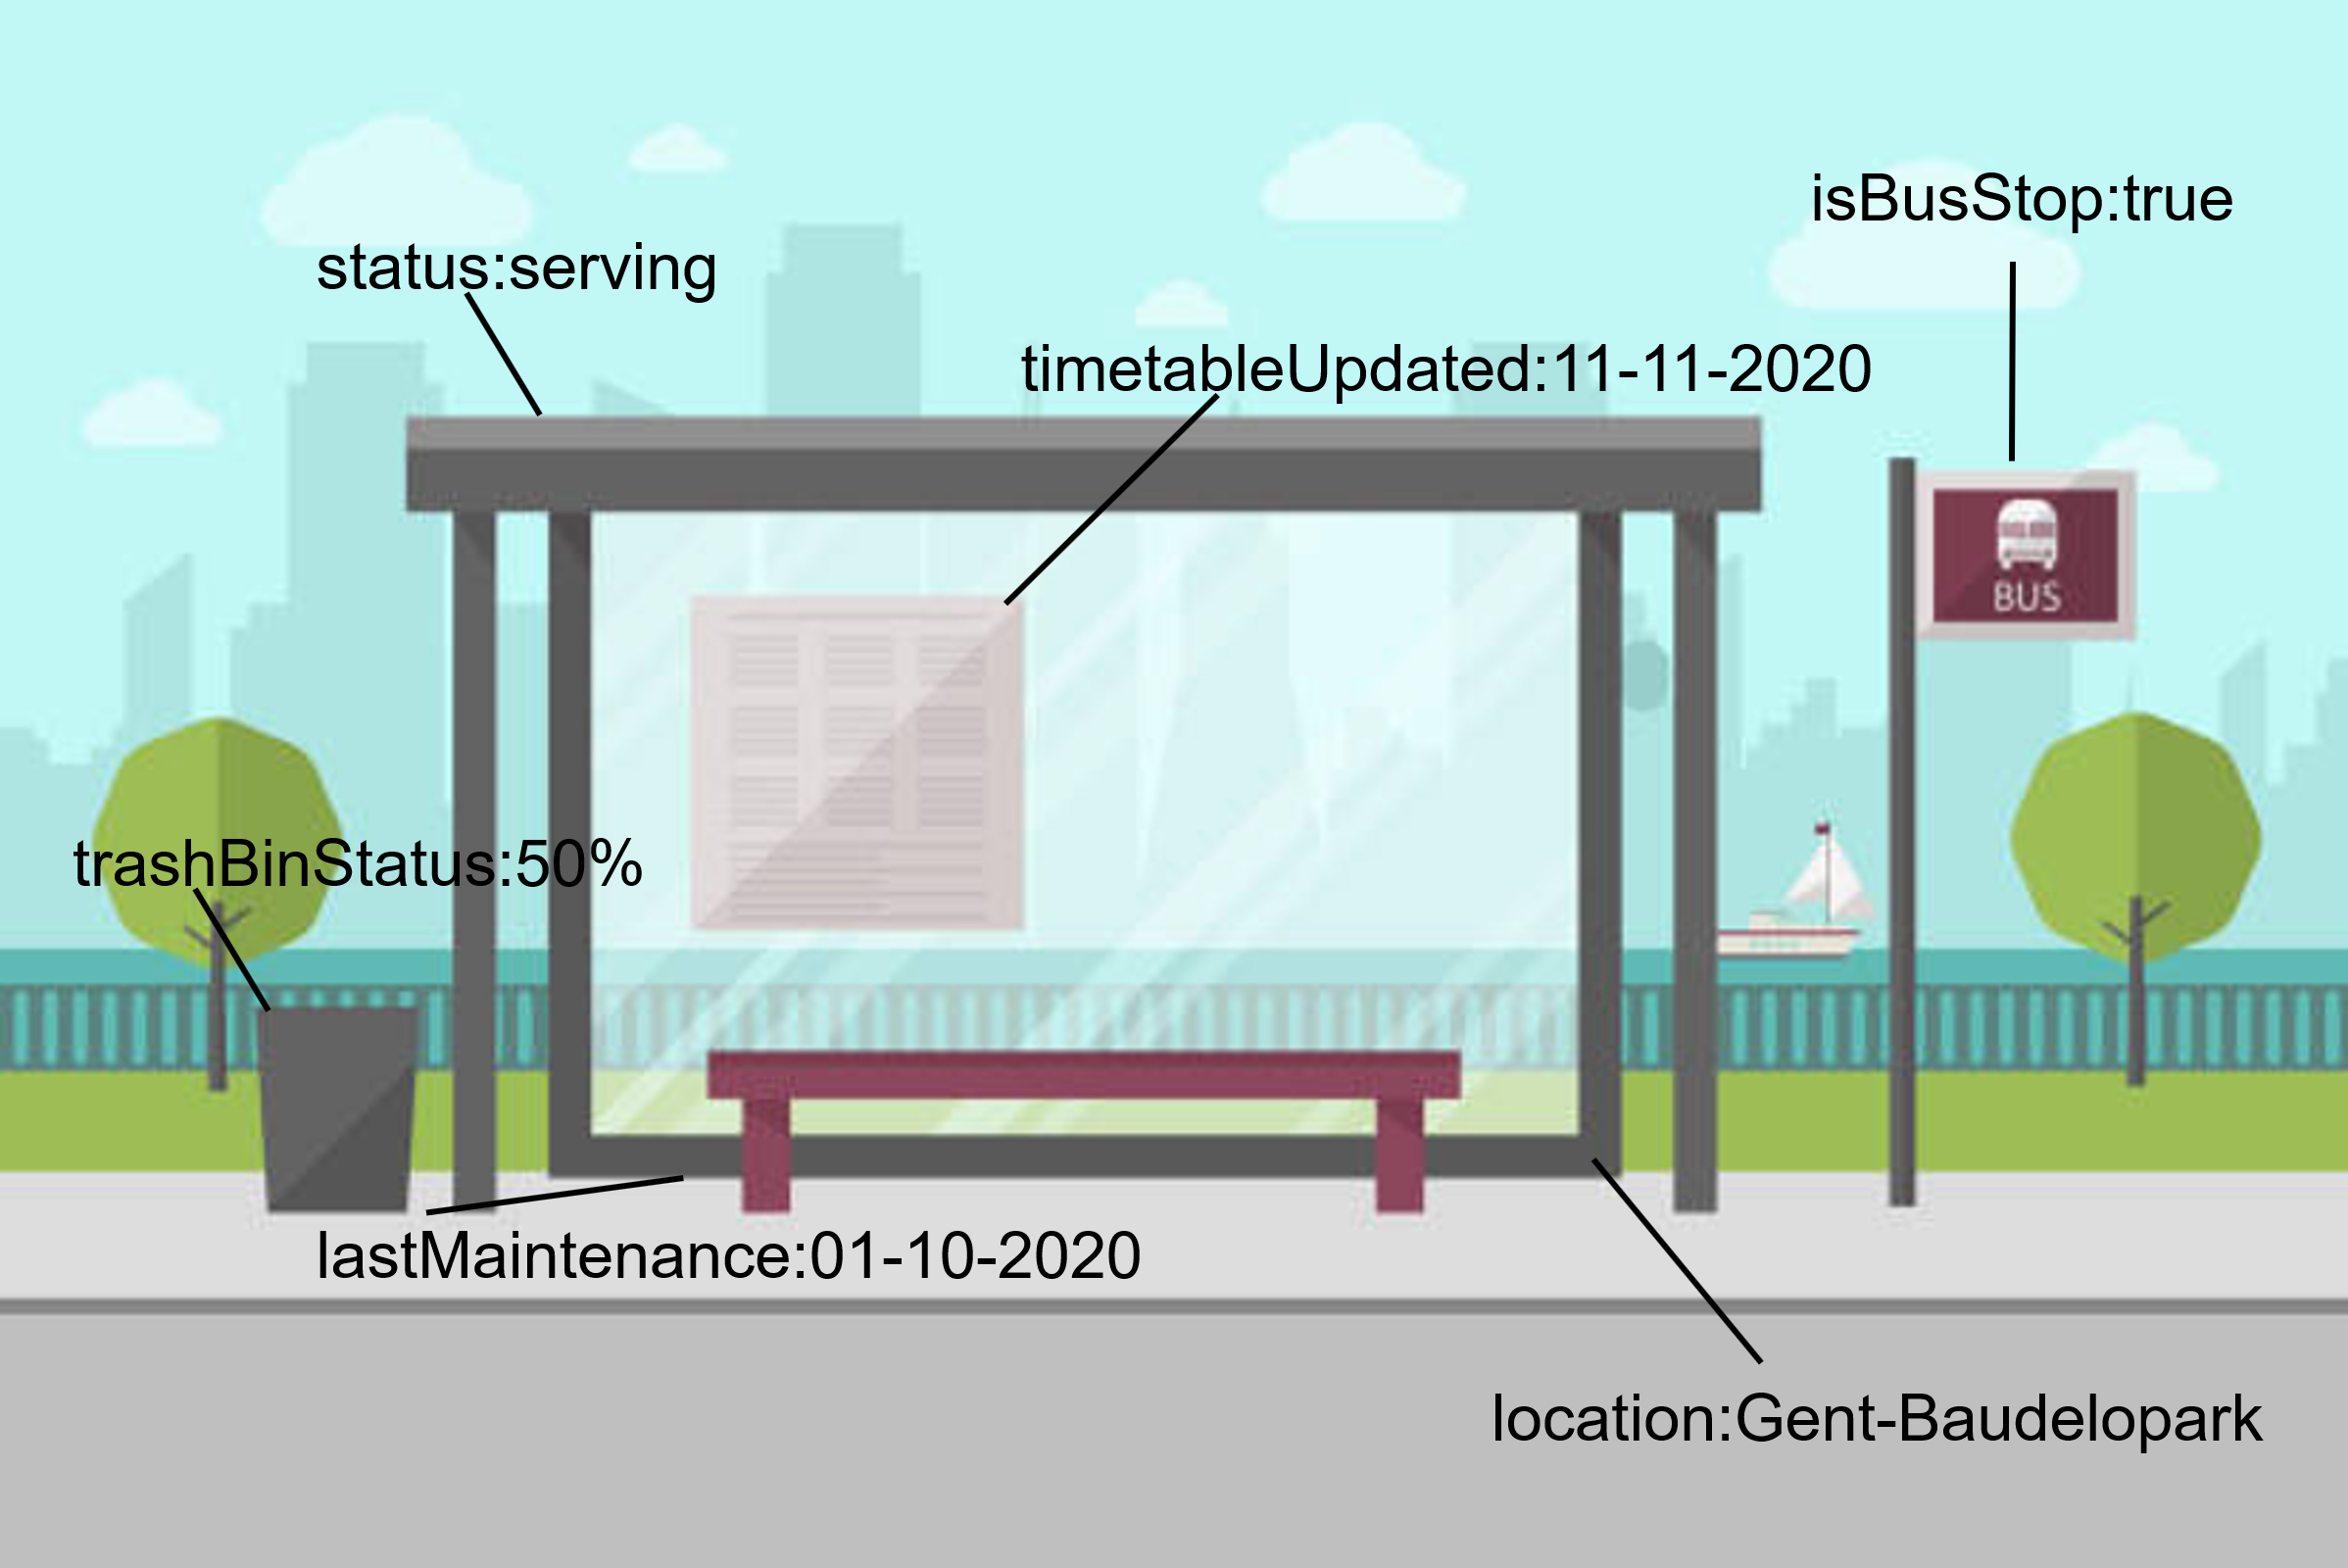
\includegraphics[scale=0.35]{images/busstation_labels.png}
		}
	\end{subfigure}
	\caption{Parameters van een infrastructuur object, gebaseerd op een figuur van istockphoto.com}
	\label{fig:busstation_labels}
\end{figure}

\section{Open Standaarden voor Linkende Organisaties}
\label{sec:OSLO}
Het Vlaams interoperabiliteitsprogramma Open Standaarden voor Linkende Organisaties (OSLO)\footnote{\url{https://data.vlaanderen.be}} is een initiatief van de Vlaamse overheid om hergebruik van gegevens te stimuleren. Het is een van de stappen die Vlaanderen neemt richting een Open Overheid met als doel een nauwere samenwerking te creëren tussen overheid en de privé sector.
Een vorige stap naar open data was het openbaar beschikbaar maken van het Grootschalig Referentiebestand (GRB). Het GRB is een digitale topografische referentiekaart van Vlaanderen waarop alle gebruikers eigen geografische gegevens kunnen aanduiden. Deze locatie gegevens van gebouwen, percelen, wegen en hun inrichting, waterlopen, spoorbanen en het wegennetwerk identificeren miljoenen objecten in Vlaanderen. Dit referentiebestand wordt gebruikt voor onder andere dispatchingtool bij hulpdiensten en het lokaliseren en intekenen van ondergrondse kabels en leidingen~\cite{wat_is_grb}. Sinds het GRB openbaar beschikbaar werd via een gegevensportaal\footnote{\url{http://opendata.vlaanderen.be}} is het gebruik ervan enorm toegenomen~\cite{grb_OD}.

Desondanks de nuttige toepassingen dat het systeem brengt, ondervinden heel wat gebruikers (private partners, bevolking en publieke administratiediensten) moeilijkheden bij het verbinden met en interpreteren van deze open data bronnen. Deze problemen met de interoperabiliteit van gegevens veroorzaken strubbelingen bij het hergebruiken van deze publieke sector informatie~\cite{opengovernment}. Om de vraag naar interoperabele gegevens te beantwoorden werd het OSLO programma opgestart dat verder bouwt op de principes van Linked Data en voldoet aan de aanbevelingen uit het \acrshort{eif}.

Het OSLO programma legt de betekenis vast van concepten, woorden en definities en hoe ze te structureren zijn in databases of softwarepakketten. Dankzij deze afspraken, omschreven in datastandaarden, kunnen semantische discussies en misverstanden worden vermeden~\cite{OSLO_handleiding}.

\subsection{OSLO services}
Informatie Vlaanderen biedt verschillende services aan waarmee het organisaties, in zowel de publieke als privé sector, op het OSLO traject helpt. Samen met de organisatie in kwestie onderzoekt het OSLO-team in hoeverre de aangeleverde informatiemodellen kunnen afgestemd worden op bestaande OSLO vocabularia. Nadat de noden voor een gegevensmodel in kaart gebracht werden, zal het team een datastandaard (of OSLO vocabularium) ontwikkelen volgens `Proces \& Methode' van OSLO\footnote{\url{https://data.vlaanderen.be/cms/Proces_en_methode_voor_de_erkenning_van_datastandaarden_v1.0.pdf}}, dat zijn richtlijnen voor het ontwikkelen van nieuwe standaarden binnen OSLO. Nadat er een gepaste datastandaard ontwikkeld of een reeds bestaande standaard toegewezen werd, wordt er ook ondersteuning geboden bij het implementatieproces.

\section{Verhoogde interoperabiliteit met OSLO}
Het doel van OSLO is om de gegevensoverdracht tussen verschillende organisaties te versnellen en automatiseren. Dit is nodig omdat de overheid meer dan duizend diensten aanbiedt aan burgers en bedrijven~\cite{OSLO_handleiding}. Deze samenwerking kost tijd en geld doordat gegevens niet interoperabel zijn. Dankzij de hulp van de experten binnen Informatie Vlaanderen die OSLO mogelijk maken, wordt de nood aan interoperabele gegevens tegemoetgekomen. Gegevens worden eenduidig gedefinieerd en hergebruikt met als resultaat meer samenhang tussen informatie en bijgevolg betere begrijpbaarheid en vindbaarheid ervan.

De huidige doelstelling bestaat erin om zoveel mogelijk gegevenssets te (her)publiceren als \acrshort{lod} met behulp van het OSLO programma. Gegevens rond nieuwe projecten kunnen vanaf nul worden opgebouwd met gestandaardiseerde gegevensmodellen. Reeds bestaande gegevenssets moeten worden omgevormd, zodat het gebruikmaakt van die standaard modellen. Hiervoor zijn tools nodig die verder in deze scriptie worden besproken.

\chapter{Linked Data}
\label{chap:intro}

Tim Berners-Lee, de grondlegger van het \acrfull{www} en oprichter van het \acrfull{w3c}, pleit al jaren voor ``raw data''\footnote{video:  \url{https://www.ted.com/talks/tim_berners_lee_the_next_web} op 10'40''}. Daarmee vraagt hij aan instellingen zoals overheden, onderzoekscentra en bedrijven om hun gegevens openbaar op het internet beschikbaar te stellen zodat het toegankelijk is voor iedereen om er onderzoek op uit te voeren~\cite{tedtalk}. Het openbaar maken van data en het zo ter te beschikking stellen voor iedereen zou wereldverbeterende inzichten moeten opleveren zoals economische groei, efficiënter gebruik van resources en een beter leefwereld voor burgers~\cite{tedtalka}.

\section{Linked Open Data}
\label{sec:linked_open_data}
Om uit al die beschikbare data op het Web inzichten te kunnen verwerven, is er nood aan hulpmiddelen die gegevens met elkaar in verbinding brengen zoals hyperlinks doen met documenten. Die hulpmiddelen samen vormen een framework, het Semantisch Web genoemd, waarmee gegevens kunnen worden gepuliceerd volgens het vijfsterrenmodel van Tim Berners-Lee. Open data krijgt vijf sterren wanneer het voldoet aan een aantal voorwaarden: de gegevens moeten online beschikbaar zijn in een open bestandsformaat, bovendien moet het gebruikmaken van de w3c\footnote{\url{https://www.w3.org/standards/}} standaarden zoals \acrfull{rdf} en SPARQL zodat anderen naar de dataobjecten kunnen verwijzen. De gegevens zelf moeten ook verwijzen naar gegevens van anderen zodat er meer context kan gecreeërd worden. Gegevens met vijf sterren worden ook wel \acrfull{lod} genoemd~\cite{opendata}.

\begin{figure}
	\centering
	\begin{subfigure}{\textwidth}
		\centering
		\centerline{
			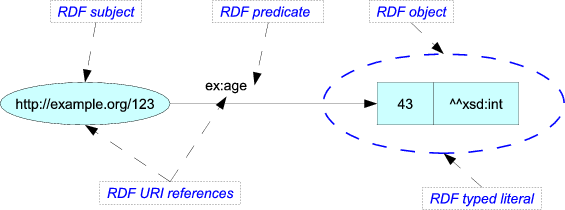
\includegraphics[scale=0.75]{images/rdfexample.png}
		}
	\end{subfigure}
	\caption{Voorbeeld van een \acrshort{rdf} graaf~\cite{rdfgraph_img}}
	\label{fig:rdf_example}
\end{figure}

\section{Resource Description Framework}
\label{sec:rdf}
\acrfull{rdf} is de open standaard die wordt gebruikt om publicatie van gegevens naar het hoogste niveau van het vijfsterrenmodel te tillen. De standaard hergebruikt het concept \acrfull{uri}\footnote{\url{https://tools.ietf.org/html/rfc3986}} waarmee objecten en concepten kunnen worden geïdentificeerd. Een URI identificeert een object en kan met andere URIs worden gelinkt zodat er context gecreëerd wordt rond dat object. Het linken van URIs gebeurt in de vorm van RDF triples: een driedelige subject-predicaat-object structuur. Deze gelinkte structuur vormt een gerichte en gelabelde graaf waarbij de takken informatie bevatten (predicaat) over de relatie tussen twee knopen (subject en object)~\cite{rdf_triple}. Figuur~\ref{fig:rdf_example} geeft een voorbeeld van hoe zo een graaf er kan uitzien met hieronder een bijhorende tekstuele representatie:

\begin{code}
\begin{minted}[breaklines]{turtle}
@prefix ex:  <http://example.org/> .
@prefix xsd: <https://www.w3.org/2001/XMLSchema#> .

<http://example.org/123> ex:age 43^^xsd:int .
\end{minted}
\caption{RDF triple in turtle formaat}
\label{code:rdftriple}
\end{code}

\acrshort{rdf} triples kunnen geserialiseerd worden in verschillende vormen. Bovenstaande representatie maakt gebruik van de Turtle syntax\footnote{\url{https://www.w3.org/TR/turtle/}}. Andere serialisatieformaten zijn JSON-LD, RDF/XML, N-triples, ...~\cite{publishingLD}.

In dit voorbeeld wordt het RDF subject, dat kan hier een persoon zijn, voorgesteld door een \acrshort{uri} die verwijst naar een andere bron die bijvoorbeeld namen van studenten bevat. Met deze triple wordt het subject uitgebreid met een leeftijd. Het RDF object in figuur~\ref{fig:rdf_example} is geen \acrshort{uri} referentie maar een `RDF typed literal' gebruikt om strings, data en, in dit geval, een getal voor te stellen. Toch kunnen objecten ook verwijzen naar een \acrshort{uri} zoals in deze uitbreiding:

\begin{code}
\begin{minted}[breaklines]{turtle}
@prefix ex:   <http://example.org/> .
@prefix xsd:  <https://www.w3.org/2001/XMLSchema#> .
@prefix foaf: <http://xmlns.com/foaf/0.1/> .

<http://example.org/123> ex:age 43^^xsd:int ;
                         foaf:knows <http://example.org/456> .
\end{minted}
\caption{RDF triple in turtle formaat - uitbreiding van Listing \ref{code:rdftriple}}
\label{code:rdftriple_uitbreiding}
\end{code}

Aan het RDF subject wordt nu door middel van het foaf:knows\footnote{\url{http://xmlns.com/foaf/spec/\#term_knows}} predicaat een RDF object gekoppeld dat gedefinieerd werd door een \acrshort{uri} referentie.
In deze uitbreiding werd gebruik gemaakt van een predicaatlijst. Met behulp van het `;'-teken kan het subject worden herhaald waarna predicaat en object kunnen variëren. 
Stel dat deze triples als document online gepubliceerd wordt in dit Turtle-formaat, dan voldoet het aan de vereisten van \acrshort{lod} omschreven in~\ref{sec:linked_open_data}.

\section{RDF vocabularium}
Om RDF-datamodellen op te bouwen zoals in het voorbeeld hierboven~(\ref{code:rdftriple_uitbreiding}), is er een \gls{ontologie} nodig. \Glspl{ontologie} zijn op voorhand gedefinieerde concepten die relaties kunnen hebben met elkaar en dat binnen hetzelfde \gls{ontologie} of met andere externe \glspl{ontologie}. Met behulp van deze documenten kan een gegevensset gemapt worden naar een \acrshort{rdf}-datamodel.
Het publiceren van een document dat een \gls{ontologie} beschrijft, gebeurt opnieuw als \acrshort{lod} door gebruik te maken van het \acrshort{rdf} framework. De term `ontologie' wordt ook vaak gebruikt om een RDF vocabularium mee aan te duiden, maar duidt een meer complexe collectie van termen aan. `Vocabularium' wordt in een lossere omgeving toegepast. Alhoewel de twee termen van elkaar verschillen is er geen duidelijk onderscheid over wanneer een dergelijk document een vocabularium of ontologie wordt genoemd~\cite{ontology}.

\subsection{RDF Schema}
RDF Schema (RDFS) is het basis RDF vocabularium waarmee andere vocabularia kunnen worden gemodelleerd. Het definieert klasses, eigenschappen en datatypes die de basis blokken vormen om andere vocabularia te definiëren~\cite{verborgh_webfundamental}. 

\subsection{Ontology Web Language}

\subsection{Voorbeeld}
Een simpel voorbeeld van een \gls{ontologie} ziet er als volgt uit:

\begin{code}
\begin{minted}[breaklines]{turtle}
@prefix owl: <https://www.w3.org/2002/07/owl#> .
@prefix rdf: <http://www.w3.org/1999/02/22-rdf-syntax-ns#> .
@prefix rdfs: <http://www.w3.org/2000/01/rdf-schema#> .
@prefix foaf: <http://xmlns.com/foaf/0.1/> .

foaf:knows a rdf:Property,
             owl:ObjectProperty ;
            rdfs:comment "A person known by this person (indicating some level of reciprocated interaction between the parties)." ;
            rdfs:domain foaf:Person ;
            rdfs:isDefinedBy foaf: ;
            rdfs:label "knows" ;
            rdfs:range foaf:Person .
\end{minted}
\caption{Voorbeeld uit de `foaf' ontologie~\cite{foaf_in_turtle}}
\label{code:foaf_ontologie}
\end{code}

Dit voorbeeld omschrijft het \textit{foaf:knows} predicaat uit codevoorbeeld~\ref{code:rdftriple_uitbreiding}. Bij het definiëren van dit concept wordt gebruik gemaakt van andere \glspl{ontologie} door via \acrshort{uri}s te verwijzen naar concepten uit andere \glspl{ontologie}. Door het concept `knows' te interpreteren wordt duidelijk dat het om een eigenschap gaat dat moet gebruikt worden binnen het domein \textit{foaf:Person}. Het object dat de eigenschap aanvaardt, wordt aangeduid met de `range' eigenschap en is in dit voorbeeld ook de klasse \textit{foaf:Person}.

Enkele veelgebruikte \glspl{ontologie} zijn:
\begin{table}[h]
\centering
\caption{vocabularia}
\begin{tabular}{ll}
rdf    & https://www.w3.org/1999/02/22-rdf-syntax-ns\#                    \\
rdfs   & https://www.w3.org/2000/01/rdf-schema\#                          \\
owl    & https://www.w3.org/2002/07/owl\#                                 \\
schema & https://github.com/schemaorg/schemaorg/blob/main/data/schema.ttl
\end{tabular}
\end{table}

\section{Probleemstelling en doel van de masterproef}
\label{sec:problem}
Zoals beschreven in Sectie~\ref{chap:interoperabele_gegevens} is er nood interoperabiliteit tussen gegevens door de verscheidene manieren waarin publieke en private sectoren hun gegevens publiceren. Deze non-interoperabiliteit resulteert in een moeilijke samenwerking tussen partijen die gegevens van elkaar gebruiken. In deze masterproef worden gegevens gerelateerd aan mobiliteit in beschouwing genomen.

Wanneer gegevens worden herpubliceerd als Linked Open Data, worden identificatoren herbruikbaar wat de interoperabiliteit tussen gegevens verhoogt. Om de principes van \acrshort{lod} te volgen, werd in deze masterproef een voorstel voor een RDF ontologie ontwikkeld die rekening houdt met objecten en eigenschappen die gebruikt worden in reeds bestaande gegevenssets van de \glspl{mobop} Blue Bike en Velo. Als tweede stap moeten deze bestaande gegevenssets, gepubliceerd in uiteenlopende datamodellen en -formaten, gemapt worden naar een RDF datamodel met behulp van die ontwikkelde ontologie.
Deze twee stappen vormen de `oprit' naar de wereld van \acrshort{lod} en wordt verder in deze scriptie de `on-boarding' van gegevens genoemd. Na deze on-boarding fase kunnen de gegevens verder hun weg vinden naar onder andere archivering en kunnen 
queries opgebouwd worden die meerdere thematisch verschillende gegevenssets aanspreken.

Er wordt, op dit moment van schrijven, in Vlaanderen al volop gewerkt aan deze wereld van \acrshort{lod} met het Vlaams interoperabiliteitsprogramma `Open Standaarden voor Linkende Organisaties' of kortweg: OSLO\footnote{https://data.vlaanderen.be/}. Dit programma ontwikkeld ontologieën om gegevens van (Belgische) overheden en bedrijven te publiceren als \acrshort{lod}. De doelstelling is om ook gegevens van \glspl{mobop} te on-boarden in het OSLO-traject.

Deze masterproef zal specifiek inzoomen op gegevenssets van Vlaamse \glspl{fietsdeelop} Blue Bike en Velo: in welk datamodel en -formaat publiceren zij hun gegevens en hoe kunnen die worden gemapt naar een RDF datamodel. Ter demonstratie worden gegevens met behulp van de ontwikkelde ontologie gemapt naar een \acrshort{rdf} datamodel en gepubliceerd als \acrlong{lod}. Tijdens het onderzoek en de implementatie wordt er zo generiek mogelijk te werk gegaan zodat in een volgende fase andere types vervoermiddelen kunnen worden geïmplementeerd.

\chapter{Het huidige speelveld rond mobiliteitsgerelateerde gegevens}

Er zijn specificaties (GBFS\footnote{\url{https://github.com/NABSA/gbfs}}, GTFS\footnote{\url{https://developers.google.com/transit/gtfs/reference}}, MDS\footnote{\url{https://github.com/openmobilityfoundation/mobility-data-specification/tree/master}}) die een zo generiek mogelijk gegevensmodel voorstellen zodat \glspl{mobop} hun gegevens op een interoperabele manier kunnen publiceren. Helaas zijn deze specificaties volgens het sterrenschema van Tim Berners-Lee geen vijf sterren waard. De gepubliceerde gegevens voldoen daarom niet aan de concepten van het European Interoperability Framework door tekortkomingen beschreven in secties~\ref{sec:GBFS} en \ref{sec:ngsi}.

Daarnaast bestaan er al \glspl{ontologie} (Mobivoc\footnote{\url{http://schema.mobivoc.org}} en OSLO mobiliteit: trips \& aanbod\footnote{\url{https://data.vlaanderen.be/doc/applicatieprofiel/mobiliteit-trips-en-aanbod}}) waarmee gegevens van \glspl{mobop} als \acrshort{lod} kunnen worden gepubliceerd. Deze vocabularia hebben beperkingen die omschreven worden in secties~\ref{sec:trips&aanbod} en \ref{sec:mobivoc} waardoor ze geen volledige oplossing bieden voor fietsdeeloperator gerelateerde gegevens. Wel kunnen deze \glspl{ontologie} gebruikt worden als basis voor een nieuwe ontologie of kan er een uitbreiding voor gemaakt worden. 

\section{General Bikeshare Feed Specification}
\label{sec:GBFS}
GBFS is een open standaard voor deelmobiliteit dat in een uniform formaat real-time gegevens publiceert. Het voordeel aan deze specificatie is dat het om een open standaard gaat en bruikbaar is door iedereen en voor verschillende toepassingen. Tussen systemen die gebruikmaken van GBFS is er interoperabiliteit, maar daarbuiten niet. Wie met de standaard werkt, wordt verplicht de gegevensset te publiceren in het JSON gegevensformaat. Hierdoor blijven semantische discussies over de betekenis van de gebruikte sleutels in het model mogelijk. Dit veroorzaakt een gebrek aan interoperabiliteit bij gegevensoverdracht tussen systemen buiten de grenzen van GBFS, zoals diensten van overheden. Zonder mapping kunnen andere systemen niet aansluiten op deze gegevens gepubliceerd in de open standaard. Daarnaast vereist de standaard geen herbruikbare identificatoren waardoor de gegevens van objecten niet uitbreidbaar zijn. 

Gegevenssets gepubliceerd volgens GBFS zouden drie sterren (\ast \ast \ast) kunnen waard zijn.
De eerste ster wordt verdiend als we veronderstellen dat dergelijke gegevenssets onder een open licentie op het web beschikbaar worden gesteld (\ast). De gegevenssets worden met de standaard gepubliceerd als JSON en zijn daarom machine-leesbaar dankzij de gestructureerde vorm (\ast \ast) en het open karakter van dat bestandsformaat (\ast \ast \ast). Doordat er geen gebruik wordt gemaakt van de open standaarden van w3c (RDF) is het niet mogelijk te refereren naar de objecten (\sout{\ast \ast \ast \ast}). De standaard is er ook niet op voorzien om verwijzingen naar andere bestaande objecten te bevatten (\sout{\ast \ast \ast \ast \ast}).

Toch lijkt het model van deze specificatie een goed startpunt te zijn om gegevens van fietsdeeloperatoren in te publiceren. GBFS bewees zichzelf reeds doordat het, op het moment van schrijven,  door verschillende operatoren wereldwijd op 452 plaatsen wordt gebruikt~\cite{GBFS_systems}. Operatoren die gebruikmaken van de standaard hier in België zijn: Donkey Republic (actief in Gent) en Bird (actief in Antwerpen). De lijst~\footnote{\url{https://github.com/NABSA/gbfs/blob/master/systems.csv}} bevat voornamenlijk operatoren die deelfietsen aanbieden. Toch zijn er ook operatoren die andere voertuigen aanbieden volgens hetzelfde \gls{deeleconomie} principe en met hetzelfde gegevensmodel. Dit is mogelijk dankzij het abstracte karakter GBFS. De GBFS standaard voorziet objecten met eigenschappen voor informatie over stations en hun real-time status, voertuigen en hun status en andere systeem eigen informatie~\footnote{\url{https://github.com/NABSA/gbfs/blob/master/gbfs.md}}.

\section{NGSI}
\label{sec:ngsi}
NGSI\footnote{\url{https://fiware-ges.github.io/orion/api/v2/stable/}} is een verzameling van gegevensmodellen voor uiteenlopende toepassingen: Smart Cities, Smart Agrifood, Smart Environment, Smart Sensoring, Smart Enery, Smart Water en andere. Een van de gegevensmodellen dat FIWARE, de organisatie achter de specificatie, ontwikkeld heeft is `Bike Hire Docking Station'. Net zoals GBFS kan dit gegevensmodel worden gebruikt door fietsdeeloperatoren om hun gegevens te publiceren in JSON-formaat. Het verschil met GBFS is dat iedere eigenschap nog extra eigenschappen heeft. Die `sub-eigenschappen' houden metadata bij voor de eigenschap zoals een timestamp. Eén van die sub-eigenschappen, misschien wel de belangrijkste, is de `value'-eigenschap die de waarde van zijn super-eigenschap bijhoudt. Verdere vergelijkingen tussen NGSI en GBFS vallen buiten de scope van deze scriptie.

Deze specificatie kan met dezelfde argumenten als die voor GBFS worden beoordeeld met drie sterren (\ast \ast \ast).

\section{NGSI-LD}
\label{sec:ngsi-ld}
NGSI-LD is gebasseerd op JSON-LD\footnote{\url{https://json-ld.org/}} en is de Linked Data versie van de klassieke NGSI gegevensmodellen. JSON-LD kan door middel van het toevoegen van een `@context'-object een JSON gegevensset beschikbaar maken als Linked Data, querybaar met een SPARQL query. Gegevenssets gepubliceerd als NGSI-LD zijn daarom vijf sterren waard (\ast \ast \ast \ast \ast).
Een NGSI-LD gegevensmodel zit anders in elkaar dan een klassiek RDF model door het invoeren van sub-eigenschappen. Daarom introduceert het een eigen vocabularium met predicaten en objecten. Zo kunnen er relaties gedefinieerd worden tussen eigenschappen van subject en die zijn sub-eigenschappen. Dat vocabularium is opgenomen in de NGSI-LD core context\footnote{\url{https://uri.etsi.org/ngsi-ld/v1/ngsi-ld-core-context.jsonld}}. In de gegevensmodellen context\footnote{\url{https://fiware.github.io/data-models/context.jsonld}} van NGSI, worden URIs beschreven voor de termen die gebruikt worden in hun modellen. Binnen het NGSI-LD ecosysteem is er dankzij die URIs interoperabiliteit. 

\section{OSLO mobiliteit: trips \& aanbod}
\label{sec:trips&aanbod}
De OSLO mobiliteit: trips \& aanbod specificatie is onderdeel van het OSLO programma beschreven in sectie~\ref{sec:OSLO}. Gezien de aard van OSLO kan een gegevensset gepubliceerd volgens dit RDF vocabularium worden beoordeeld met vijf sterren (\ast \ast \ast \ast \ast). Het vocabularium voorziet allerhande termen voor gegevensuitwisseling over door personen uitgevoerde reizen en de mobiliteitsdiensten die ze daarvoor ter beschikking hebben~\cite{oslomobiliteit}. Dit lijkt een goed kandidaat-gegevensmodel waarmee gegevens van fietsdeeloperatoren kunnen worden gepubliceerd. De klassen en eigenschappen beschreven door het vocabularium zijn echter beperkt. De RDF termen beschrijven hoofdzakelijk zeer low level concepten en begrippen zoals aanbieder, mobiliteitsdienst, prijsplan, reiziger, route enz...~\footnote{\url{https://data.vlaanderen.be/doc/applicatieprofiel/mobiliteit-trips-en-aanbod\#overview}} Om gegevens van fietsdeeloperatoren te publiceren is er meer nood aan RDF termen gelijkaardig aan de properties van GBFS.

\section{MobiVoc: Open Mobility Vocabulary}
\label{sec:mobivoc}
Deze specificatie maakt ook gebruik van RDF. Gegevens gepubliceerd met dit RDF vocabularium hebben potentieel om vijf sterren (\ast \ast \ast \ast \ast) waard te zijn. Mobivoc profileert zich als een vocabularium voor toekomstgerichte mobiliteit. Hiermee lijkt ook dit vocabularium een goede kandidaat voor het publiceren van gegevens van fietsdeeloperatoren als LOD. Het vocabularium bevat een ruim assortiment aan RDF termen zoals `bicycle parking station' dat een subklasse is van `parking facility'. Daarnaast bevat het ook termen om eigenschappen van voertuigen en stations te modelleren zoals de real-time capaciteit. 

Hetgeen dat hier mist is een connectie met OSLO zodat er kan gelinkt worden naar reeds bestaande gegevenssets in Vlaanderen. Op die manier kunnen nieuwe en bestaande fietsenstallingen voor deelfietsen gelinkt worden aan adressen, plaatsen of openbare gebouwen die reeds als LOD objecten ter beschikking worden gesteld met de OSLO vocabularia. 